\chapter{Scalable Algorithm Design}

\section{Introduction}
\par
What is big data? There are a lot of examples of vast repositories of data (the Web, Physics, Astronomy, Finance), their main characteristics are great \textbf{volume}, high growing \textbf{velocity} and \textbf{variety}.
\par\noindent
Generally, the bigger is the amount of data the smaller is the importance of the algorithm used. \textbf{With more data, accuracy of different algorithms converges}.
\par\noindent
The "Map Reduce" programming model is used to work with big data, it is a distributed programming model designed for large-scale data processing to run on clusters of commodity hardware.

\section{Key Principles}
\subsection*{Scale out instead of scale up}
For data intensive workloads, a large number of commodity servers is preferred over a small number of high-end servers.
I/O is very slow compared to processing speed therefore using more HDD in parallel instead of just one can improve performances. Moreover a sharing approach is better than shared nothing but sharing is difficult for various reasons (Synchronization, Deadlocks, Bandwidth).
\subsection*{Failures are the norm, not the exception}
Failures are mostly due to the scale and shared environment. There can be different types of failures (Permanent or Transient) coming from different sources (Hardware, Software, Cooling, Electrical).
\subsection*{Move processing to the data}
Generally, data intensive workloads are not processor demanding (no more HPC) so the \textbf{network becomes the bottleneck}. The framework exploits the \textbf{data locality principle} in order to assume processing and storage nodes to be collocated. \textbf{Distributed file systems} are necessary.
\subsection*{Process data sequentially, avoid random access}
Relevant datasets can be too large to fit in memory therefore \textbf{disk performance is a bottleneck} and systems are designed for batch processing involving mostly full scans of the data (organize computation in sequential reads).
\subsection*{Hide system-level details}
The framework abstracts away the distributed part of the system but in-depth knowledge of the framework is key.
\subsection*{Seamless scalability}
Scalability can be defined along two dimensions, in terms of \textbf{data}: given twice the amount of data, the same algorithm should take no more than twice as long to run; in terms of \textbf{resources}: given a cluster twice the size, the same algorithm should take no more than half as long to run.
The \textbf{embarrassingly parallel problem} aims at defining problems that require independent computation on fragments of the dataset.

\section{The Programming Model}
\subsection{Functional programming roots: Map and Fold}
Map and Fold are high order functions: functions that accept other functions as arguments.
\subsubsection{Map phase}
Given a list, Map takes as an argument a function \textit{f} (that takes a single argument) and applies it to all the elements in a list.
\subsubsection{Fold phase} 
Given a list, fold takes as arguments a function \textit{g} (that takes two arguments) and an initial value (an accumulator).The function is first applied to the initial value and the first item in the list, then the result is stored in an intermediate variable, which is used as an input together with the next item to a second application of g. The process is repeated until all items in the list have been consumed.
\newline\newline
Map can be seen as a transformation over a dataset. This transformation is defined by f. Each application to an element of the dataset happens in \textbf{isolation} so that the process can be parallelized.
\par
Fold can be seen as an aggregation operation defined by g. If we can group the elements of the list also this phase can proceed in parallel (remember about data locality).
\par
Associative and commutative operations allow performance gains through local aggregation and reordering.
\subsection{Hadoop MapReduce}
In Hadoop, Map corresponds to the map operations and Reduce to the fold one. The framework coordinates the two phases and aggregates (\textbf{group}) intermediate results in parallel.
\par
Key-Value pairs are the basic data structure. The programmer defines a mapper and a reducer as follows:
\[
\textit{map: (k1,v1) $\rightarrow$ [(k2, v2)] \qquad reduce: (k2, [v2]) $\rightarrow$ [(k3, v3)]}
\]
Between the map and reduce phases there is a parallel "group by" operation on intermediate keys. Intermediate data arrive at each reducer in order but there is no order across reducers. Intermediate keys are not stored on the distributed file system but on the local disk of each machine in the cluster.
\subsection{Example: word counter}
The mapper takes an input key-value pair, tokenizes the line and emits the intermediate key-value pairs: the word is the key and the integer is the value.
\par
The framework guarantees that all values associated with the same key are brought to the same reducer.
\par
The reducer receives all values associated to some keys, sums the value and writes the output key-value pairs: the key is the word and the value is the number of occurrences.
\subsection{Combiners}
Combiners are a general mechanism to reduce the amount of intermediate data and avoid huge network traffic (mini-reducers).
\par
Combiners are defined as follows:
\[
\textit{combiner: (k2, [v2]) $\rightarrow$ [(k2, v2)]}
\]
They have the same input as Reducers and the same output as Mappers.
\par
For commutative and associative operations Reducers code and Combiners code may be interchangeable but this is not true in the general case.
\begin{figure}[h!]
	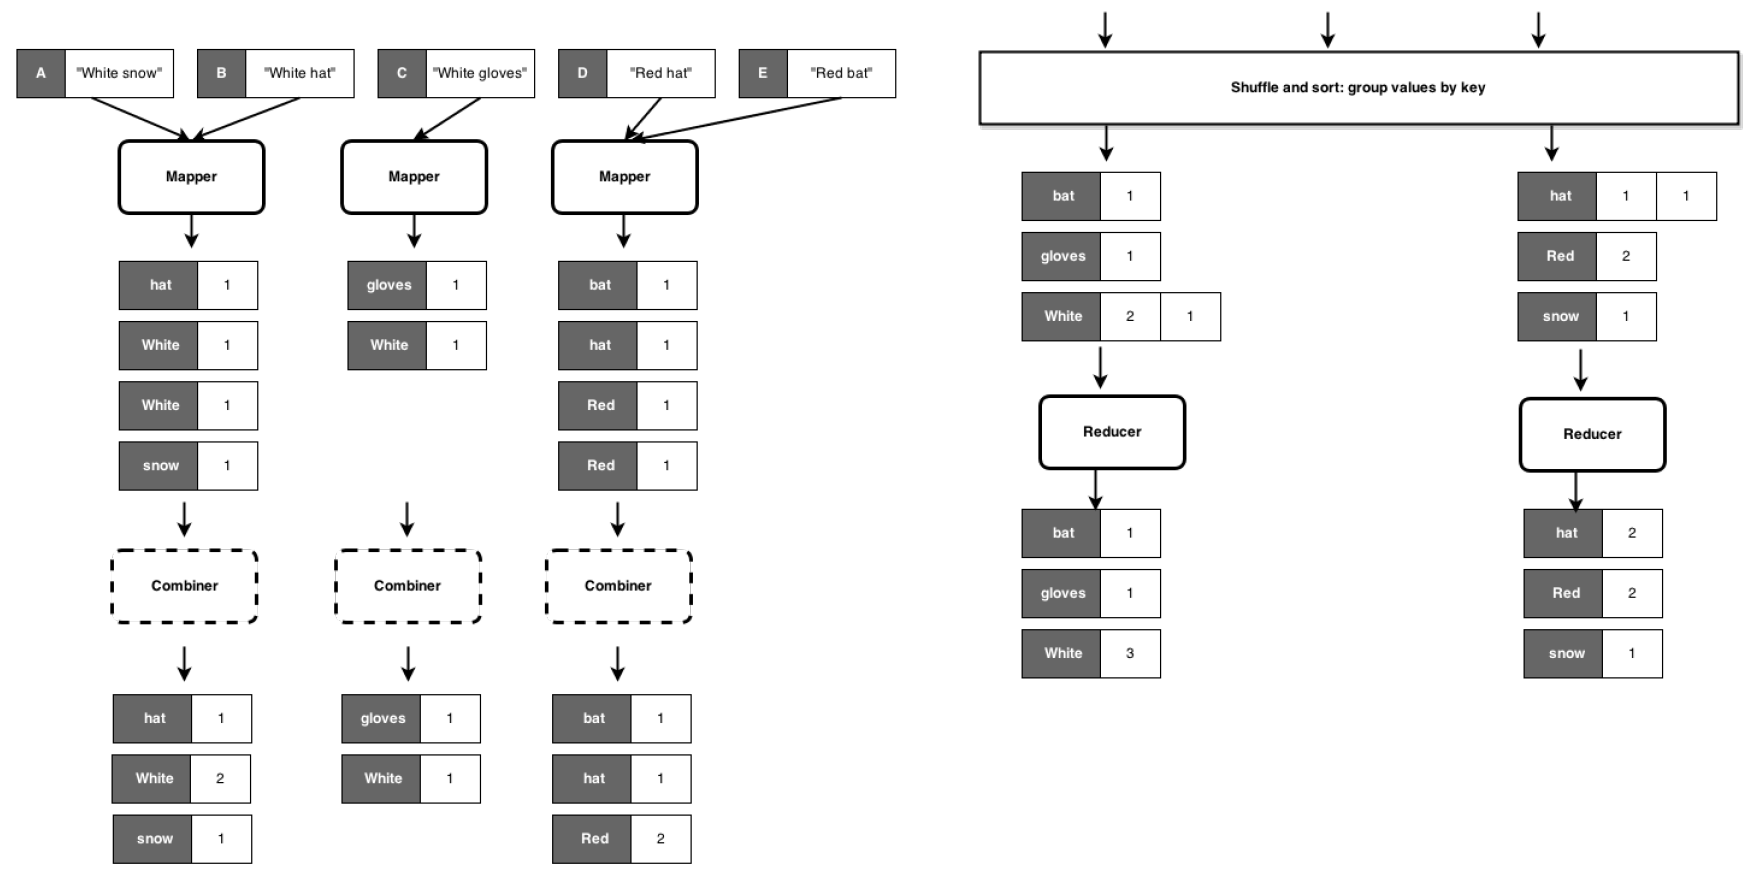
\includegraphics[width=\linewidth]{images/combiners.png}
	\caption{\textit{Word count using combiners.}}
\end{figure}
\subsection{Example: computing the mean}
We use an \textbf{identity mapper} which groups and sorts appropriately the input. Reducers keep track of the running sum and the number of integers encountered. The mean is emitted as the output of the reducer.
\par
The mean operation is not distributive hence a combiner cannot output partial means. 
\begin{figure}[h!]
	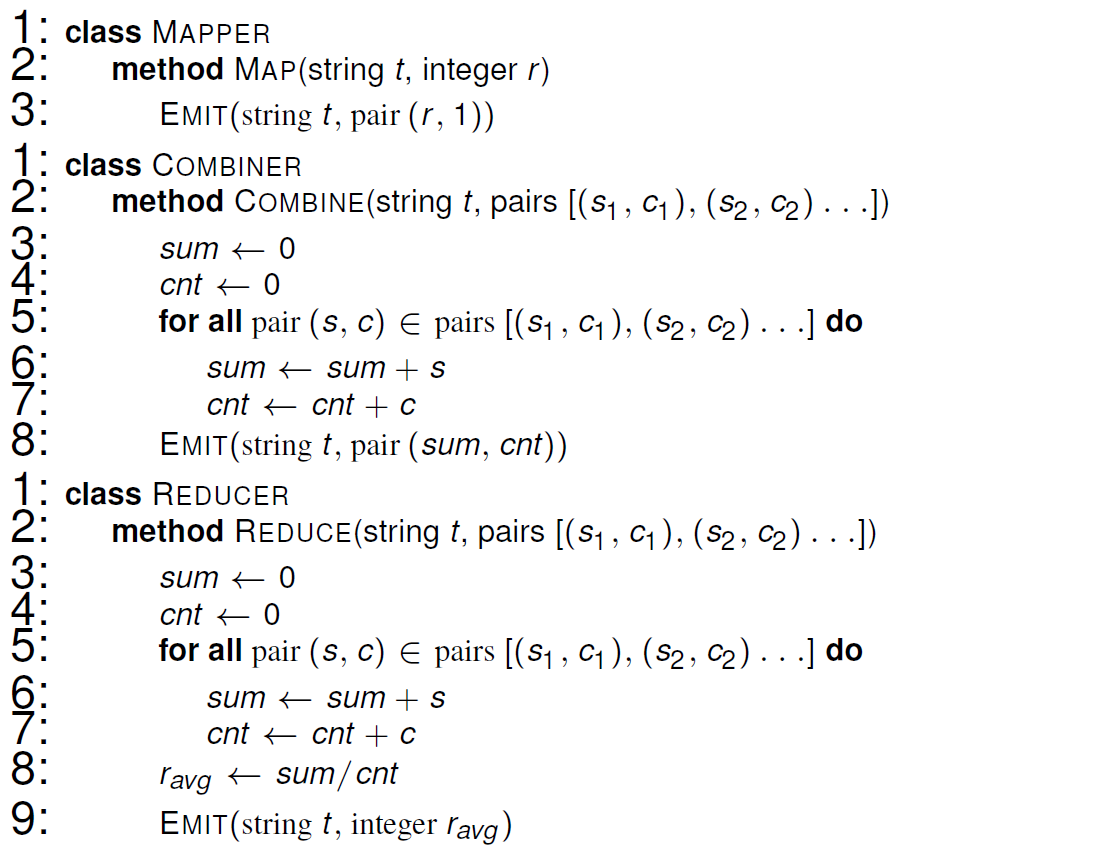
\includegraphics[width=\linewidth]{images/meanpseudocode.png}
	\caption{\textit{Pseudo-code to find the mean using combiners.}}
\end{figure}
%\captionof{figure}{pseudo code to find the mean}
\section {Basic Design Patterns}
\subsection{Algorithm design}
Developing algorithms involve preparing the input data, implementing the mapper and the reducer and, optionally, designing the combiner and the partitioner.
\par
Some of the aspects that can be controlled are: \textbf{the sort order} of intermediate keys (the order in which a reducer will encounter them) and \textbf{the partitioning of the key space} (the set of keys that will be encountered by a reducer). Moreover, the state can be preserved across multiple input and intermediate keys in mappers and reducers.
\par
Aspects that are not under the control of the designer are:
\begin{itemize}
	\item Where a mapper or a reducer will run;
	\item When a mapper or a reducer begins or finishes;
	\item Which key-value pairs are processed by a specific mapper or reducer;
\end{itemize}
\subsection{Local aggregation: In-Memory combiners}
In the context of data-intensive distributed processing, the most important aspect of synchronization is the \textbf{exchange of intermediate results} because network and disk latencies are expensive (Hadoop writes intermediate results to disk to be more fault tolerant). The use of combiners and preserving state across inputs reduces the number and size of key-value pairs to be shuffled.
\par
Combiners can be costly in terms of both CPU and I/O, \textbf{In-Mapper Combiners} could improve the performance by using an associative array (dictionary of key-value pairs) to cumulate intermediate results.
\par
To further improve the algorithm\footnote{A Java mapper object is created for each map task, the JVM reuse must be enabled.} the state can be preserved within and across calls to the map method by using \textbf{Initialize} (creates an across-map persistent data structure) and \textbf{Close} (emits intermediate key-value pairs only when all map tasks scheduled on one machine are done).
\begin{figure}[h!]
	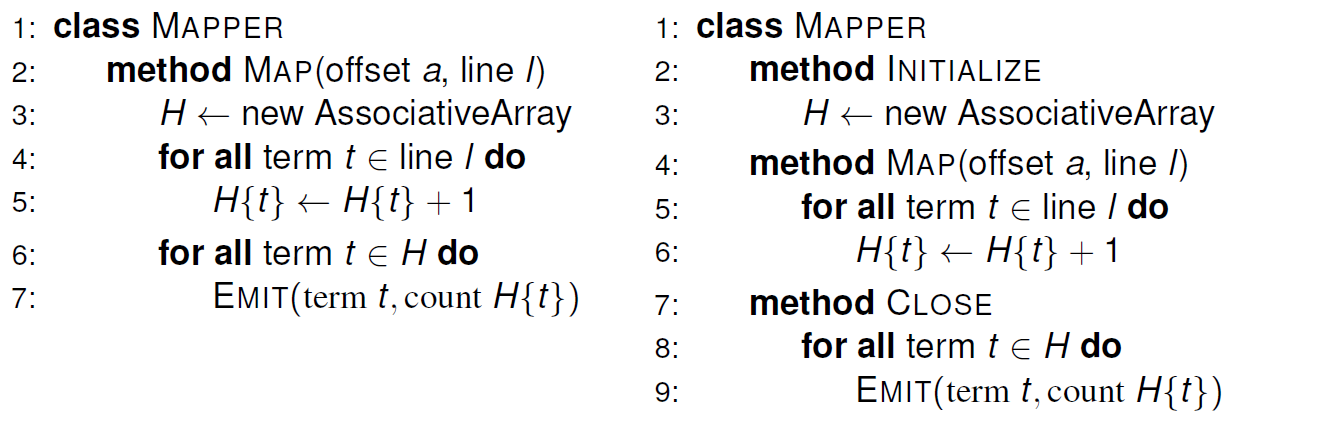
\includegraphics[width=\linewidth]{images/inmappercombiners.png}
	\caption{\textit{In-Memory combiners for the word count and mean problems.}}
\end{figure}
\par
In-Memory combiners are a \textbf{trade-off between memory usage and I/O}, the extent to which efficiency can be increased depends on the size of the intermediate key space. In-Memory combining breaks the functional programming paradigm due to state preservation, this implies that algorithm behaviour might depend on the execution order (works well with commutative/associative operations).
\par\noindent
Furthermore, it strictly depends on having enough memory to store intermediate results (possible solution: \textbf{block and flush}). Memory is an issue especially in hadoop because it is based on java and the JVM garbage collector doesn't always perform well.
\subsection{Pairs and stripes}
A common approach in MapReduce is to build complex keys (\textit{Pairs}) or values (\textit{Stripes}).
\subsubsection{Problem: Building word co-occurence matrices for large corpora}
The co-occurrence matrix is a square $n\times n$ matrix M. A cell $m _{ij}$ contains the number of times the word $w_i$ co-occurs with the word $w_j$ within a specific context (a sentence, a paragraph, a window of \textit{m} words).
\par\noindent
\textit{This matrix is useful to estimate the distribution of discrete joint events from a large number of observations.}
\par\noindent
The space requirement is $O(n^2)$ so the matrix could be bigger than the available memory (if the matrix is symmetric the space can be optimized).
\subsubsection{The pairs approach}
The mapper emits key-value pairs with \textbf{each co-occurring pair as the key} and the integer one (the count) as the value.
\par\noindent
The reducer receives pairs of co-occurring words (this \textbf{requires modifying the partitioner}) and computes the absolute count of the joint event. Then it emits the pair and the count (the cell of the matrix).
\subsubsection{The stripes approach}
The mapper stores co-occurrence information in an associative array, then it emits key-value pairs with words as keys and \textbf{the corresponding array as values}.
\par\noindent
The reducer receives all the arrays associated to the same word and performs an element-wise sum, then it emits the key-value pair in the form of word, associative array (the row of the matrix).
\begin{figure}[h!]
	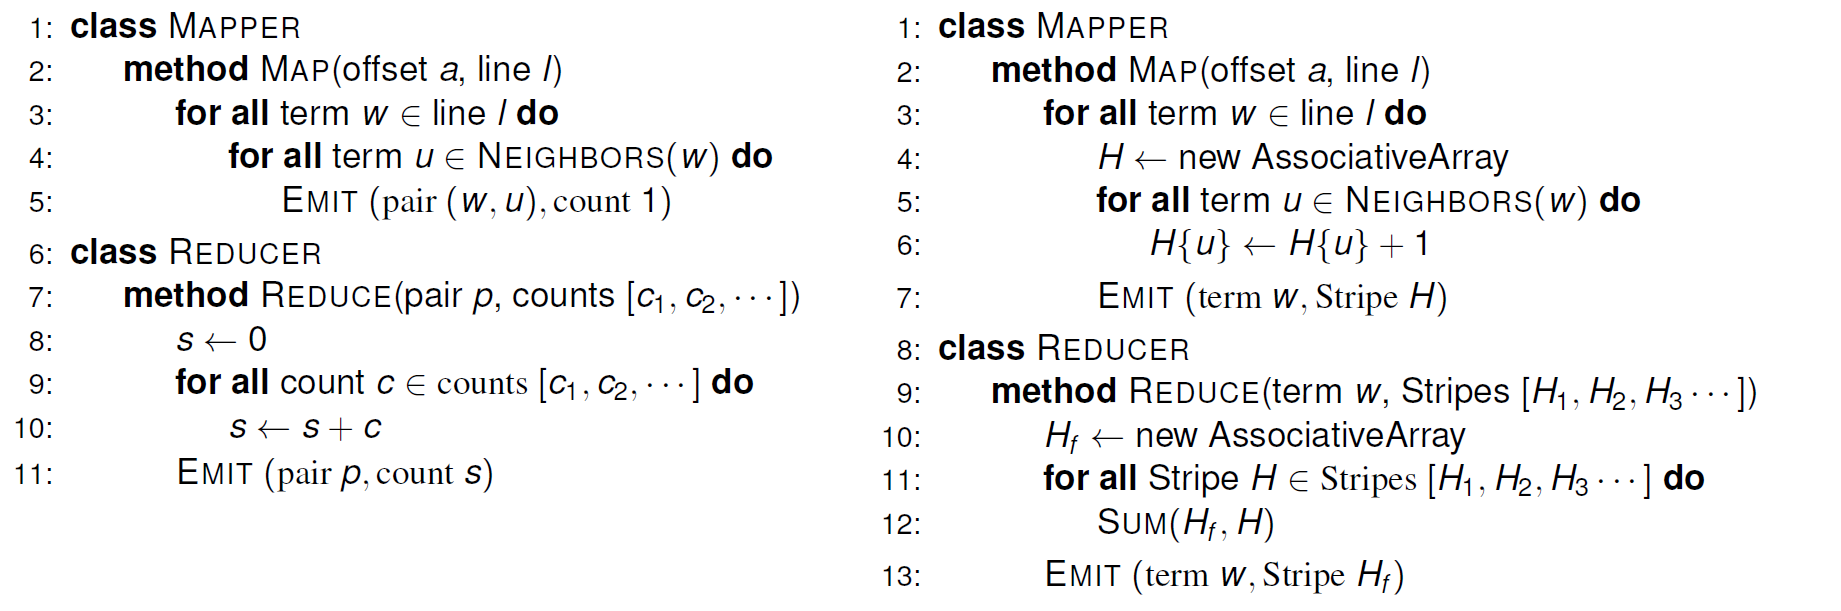
\includegraphics[width=\linewidth]{images/pairsandstripes.png}
	\caption{\textit{The pairs approach (left) and the stripes approach (right).}}
\end{figure}
\subsubsection{Pairs-stripes comparison}
Generally, the pairs approach generates a large number of key-value pairs over the network, \textbf{the benefit of combiners is limited} as it is less likely for a mapper to process multiple occurrences of a word. \textbf{It does not suffer of memory paging problems}.
\par\noindent
The stripes approach is more compact as it generates fewer intermediate keys but \textbf{the values have serialization/deserialization problems}. \textbf{It greatly benefits from combiners but may suffer of memory paging problems}.
\subsection{Order inversion}
\subsubsection{Problem: Building relative co-occurrence matrix}
The problem is similar as before but instead of absolut counts we need relative frequencies $f(w_j|w_i)$ because the word $w_i$ may co-occur frequently with word $w_j$ simply because one of the two is very common. Formally we compute:
\begin{equation*}
	f(w_j|w_i) = \dfrac{N(w_i, w_j)}{\sum_{w'}N(w_i, w')}
\end{equation*}
Where $N(\cdot,\cdot)$ is the number of times a co-occurring word pair is observed.
\newline
\par\noindent
With the stripes approach, in the reducer, the sum of all words that co-occur with $w_i$ (the denominator, \textit{marginal}) is available from the associative array.
\par
With the pairs approach we need to preserve the state in the reducer using a buffer in memory accumulating the count of all the words that co-occur with $w_i$.
\subsubsection{A basic approach}
We must \textbf{define the sort order of the pair} so that the keys are first sorted by the left word and then by the right word. In this way we can detect if all pairs associated with a word have been seen and use the in-memory buffer to compute the relative frequencies.
\par
We must \textbf{define an appropriate partitioner} so that all pairs with the same left word are sent to the same reducer. The default partitioner is based on the hash value of the intermediate key, modulus the number of reducers (for complex keys, the raw byte representation is used to compute the hash value).
\newline
\par
In order to implement this approach we need the to emit a special key-value pair $(w_i, *)$ to represent the marginal calculated by the combiner.
\par\noindent
The sort order of the intermediate key must be controlled so that the special key-value pair is processed first (define a custom partitioner).
\par\noindent
Preserve state (marginal) acrossmultiple keys in the reducer.
\par
The memory requirements are minimal because only the marginal (an integer) needs to be stored (no scalability bottleneck).
